\documentclass[conference]{IEEEtran}
\usepackage[english]{babel}
\usepackage{geometry}
\usepackage{amsmath}
\usepackage{amsthm}
\usepackage{graphicx}
\usepackage{caption}
\usepackage[utf8]{inputenc}


%%%%%%%% SUB-FIGURE PACKAGE
\usepackage{subcaption}

%%%%%%%% MULTI-COLUMNS PACKAGE
\usepackage{multicol}

%%%%%%%% PERSONAL COMMANDS
\usepackage{amssymb}

%%%% Important sets
\renewcommand{\O}{\mathbb{O}}
\newcommand{\N}{\mathbb{N}}
\newcommand{\Z}{{\mathbb{Z}}}
\newcommand{\Q}{{\mathbb{Q}}}
\newcommand{\R}{{\mathbb{R}}}

%%%% Usual operations
\newcommand{\pow}[2]{#1^{#2}}
\newcommand{\expp}[1]{e^{#1}}
\newcommand{\fst}{\mathrm{fst}}
\newcommand{\snd}{\mathrm{snd}}

%%%% Lambda Calculus
\newcommand{\dneq}{\,\, \# \,\,}
\newcommand{\prm}[1]{\mathrm{\mathbf{#1}}}
\renewcommand{\S}{\prm{S}}
\newcommand{\I}{\prm{I}}
\newcommand{\K}{\prm{K}}
\newcommand{\ch}[1]{\ulcorner #1 \urcorner}

%%%% Ordinal Lambda Calculus
\newcommand{\ordAlph}{\Sigma_{\text{Ord}}}
\newcommand{\termOrd}{\text{Term}_\text{Ord}}
\newcommand{\fl}{\mathrm{fl}}
\newcommand{\sk}{\mathrm{sk}}

%% Superscript to the left
% https://latex.org/forum/viewtopic.php?t=455
\usepackage{tensor}
\newcommand{\app}[3]{\tensor*[^{#1}]{\left(#2, #3\right)}{}}

%%%% Make optional parameter
% https://bit.ly/3jVGRwQ
\usepackage{xparse}

%%%% Statistics
\NewDocumentCommand{\E}{o m}{
  \IfNoValueTF{#1}
  {\mathbb{E}\left[#2\right]}
  {\mathbb{E}^{#1}\left[ #2\right]}
}
\NewDocumentCommand{\V}{o m}{
  \IfNoValueTF{#1}
  {\mathrm{Var}\left[#2\right]}
  {\mathrm{Var}^{#1}\left[ #2\right]}
}
\RenewDocumentCommand{\P}{o o m}{
  \IfNoValueTF{#1}
  {\IfNoValueTF{#2}
    {\mathrm{P}\left(#3\right)}
    {\mathrm{P}^{#2}\left(#3\right)}}
  {\IfNoValueTF{#2}
    {\mathrm{P}_{#1}\left(#3\right)}
    {\mathrm{P}_{#1}^{#2} \left(#3\right)}}
}

%%%% Lambda Calculus
\NewDocumentCommand{\cx}{o}{
  \IfNoValueTF{#1}
  {\left[\quad\right]}
  {\left[\, #1 \,\right]}
}

%%%% Create absolute value function
% https://bit.ly/33Rkq6H
\usepackage{mathtools}
\DeclarePairedDelimiter\abs{\lvert}{\rvert}%
\DeclarePairedDelimiter\norm{\lVert}{\rVert}%
\makeatletter
\let\oldabs\abs
\def\abs{\@ifstar{\oldabs}{\oldabs*}}
%
\let\oldnorm\norm
\def\norm{\@ifstar{\oldnorm}{\oldnorm*}}
\makeatother

%%%%%%%% LOGIC TREES
\usepackage{prftree}

%%%%%%%% SPLIT EQUATIONS
% https://bit.ly/33P1OUM
\allowdisplaybreaks

%%%%%%%% FLOAT SPECIFIER
% https://bit.ly/30Wi4BC
\usepackage{float}

%%%%%%%% TO USE SHORT COMMANDS FOR VECTOR LINES
\usepackage{esvect}

%%%%%%%% DIFFERENT FONTS FOR MATH
\usepackage{mathrsfs}

%%%%%%%% FOOTNOTE STUFF
\renewcommand{\thefootnote}{\fnsymbol{footnote}}



%%%%%%%% MARGIN
\geometry{verbose, letterpaper, tmargin=3cm,
  bmargin=3cm,lmargin=2.5cm,rmargin=2.5cm}

%%%%%%%% PARAGRAPH SETTINGS
% https://bit.ly/36WrtN4
\setlength\parindent{0pt}

% https://bit.ly/371dvto
\setlength{\parskip}{5pt}

%%%%%%%% HYPERREF PACKAGE
\usepackage{hyperref}
\hypersetup{linkcolor=blue}
\hypersetup{citecolor=blue}
\hypersetup{urlcolor=blue}
\hypersetup{colorlinks=true}


%%%%%%%% BIB-LATEX STUFF
\usepackage[style=ieee,
            bibstyle=ieee,
            citestyle=ieee,
            hyperref=true,
            backend=biber]{biblatex}
\addbibresource{ref.bib} %Put relative path to ref

%%%%%%%% DEFINITION AND THEOREM DEFINITIONS
\theoremstyle{definition}
\newtheorem{definition}{Definition}[section]

\theoremstyle{remark}
\newtheorem{remark}{Remark}

\theoremstyle{remark}
\newtheorem{question}{Question}

\newtheorem{theorem}{Theorem}[section]


%%%%%%%% CODE RENDERING !!! UNCOMMENT IF NEEDED !!!
% Compile with flag -shell-escape
%\usepackage{minted}

%%%%%%%% START DOCUMENT
\title{Experiments in Deep Learning}

\author{\IEEEauthorblockN{Juan Sebastián Cárdenas-Rodríguez}
  \IEEEauthorblockA{\textit{Department of Mathematical Sciences} \\
    \textit{EAFIT University}\\
    Medellín, Colombia \\
    jscardenar@eafit.edu.co} \and \IEEEauthorblockN{David Plazas}
  \IEEEauthorblockA{\textit{Department of Mathematical Sciences} \\
    \textit{EAFIT University}\\
    Medellín, Colombia \\
    dplazas@eafit.edu.co} }


\begin{document}
\maketitle

%%%%%%%%%%%%%%%%%%%%%%%%%%%%%
\begin{abstract}
  This work presents results of experiments of some artificial intelligence
  techniques. The work begins comparing the performance of a multilayer
  perceptron in two scenarios: using a complete dataset andd using a synthesized
  dataset by means of an autoencoder. The complete dataset worked better for the
  classification task. Then, the results of training a LeNet5 architecture for
  the MNIST hand-written digits dataset are presented, showing outstanding
  results for a fair number of epochs. Finally, an intial approach to the GANs
  architecture was done by two approaches: a GAN for the MNIST dataset and an
  StyleGAN for generating and mixing styles in humand-like and anime-like faces.
  The last part, using state-of-the-art implementations with \texttt{CUDA}.
\end{abstract}

\begin{IEEEkeywords}
  Autoencoders, convolutional networks, GAN, StyleGAN2, MNIST, CUDA.
\end{IEEEkeywords}
%%%%%%%%%%%%%%%%%%%%%%%%%%%%%

All the source can be found in \href{https://bit.ly/3qCUuVv}{this Github
  repository}. All the source code was tested using \texttt{Julia 1.5.3} and
\texttt{Python 3.9.0}.

\section{Introduction}
In this work, different experiments realized, surrounding deep learning, for the
Artificial Intelligence course of "Universidad EAFIT" are shown.

In Section \ref{sec:meth} a brief introduction of the architecture and
experiments realized are explained, in Section \ref{sec:res} the results for the
conducted experiments are shown and in Section \ref{sec:conc} the conclusions
for each experiment are presented.

\section{Methodology}\label{sec:meth}
\subsection{Autoencoder}
The general ideas for the autoencoder were studied during the class and they are
also briefly described in the course book. The autoencoders are a powerful tool
for synthesizing information of a given input, reducing its dimensions. The most
simple encoding architecture is a multilayer perceptron using only one hidden
layer and using the same input as output.

In our specific case, the autoencoder was used for reduction of the input
dataset, mapping the original inputs into a 2-dimensional feature space. Then,
the reduced dataset was compared with the original one by training the same
classification task as in our previous work, using the best hyperparameters.

\subsection{LeNet5}
The general representation of the LeNet5 architecture is presented in Fig.
\ref{fig:lenet5} and all the details can be found in its seminal paper in
\parencite{lecun1998gradient}. Note that this architecture can be ``divided''
into a convolutional component and a dense component, the former refers to an
extraction of spatial features through filtering; the latter is designed to
classify the input image according to all the feature extraction in the
convolutional layers.

\begin{figure*}
  \centering 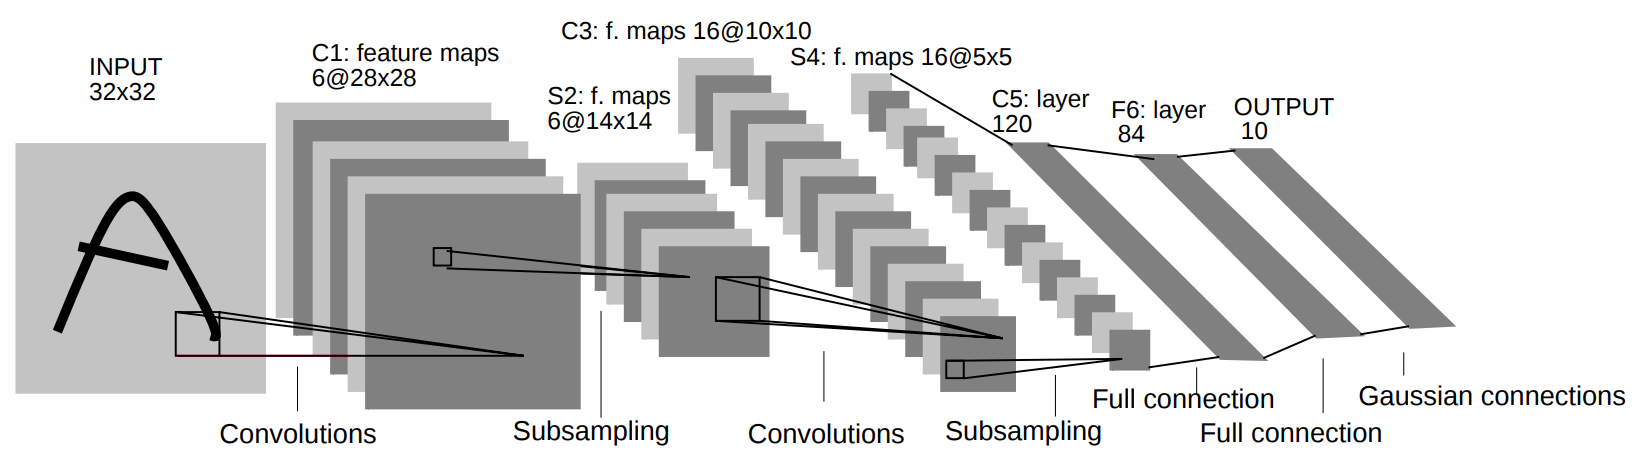
\includegraphics[width=\textwidth]{figs/letnet5.png}
  \caption{LeNet5 architecture (taken from \parencite{lecun1998gradient}).}
  \label{fig:lenet5}
\end{figure*}

\subsection{GAN}
The Generative Adversarial Network (GAN) was extracted from the implementation
available in \href{https://bit.ly/39Wwirg}{this link}, and adapted for the MNIST
dataset (originally for the Fashion-MNIST database). The general goal behind the
GAN architecture is to construct a generator and a discriminant, such that the
generator always attempts to cheat the discriminant by generating better data on
each training iteration. More specifically, the objective of the generator is to
minimize the probability of cheating and the discriminant aims to maximize the
probability of a correct classification.

\subsection{StyleGAN}
The architecture behind the StyleGAN used in this work was initially proposed in
\parencite{karras2019style} and then improved to the second version in
\parencite{karras2020analyzing}. The implementation and some documentation can
be found in \href{https://github.com/NVlabs/stylegan2}{this repository}, where
they also offer a set of pre-trained StyleGAN architectures for different
datasets. We focused on two networks: one trained for the FFHQ human face
dataset, and other trained for generating Anime Portraits. An excellent gallery
of the applications of StyleGAN2 in different types of images is presented in
\href{https://github.com/justinpinkney/awesome-pretrained-stylegan2}{this
  repository}.

The installation of the suggested repository is really awkward, as some
dependencies are hard to find for each system. For this, the authors suggest
having a mirror of \texttt{Ubunt 18.04} and following the tutorial given
\href{https://bit.ly/2VUagNB}{by this link}.

\subsection{MNIST}
The MNIST dataset contains 70k handwritten digits. This digits are represented
by images of size $28 \times 28$ using a grey scale of colors. It was originally
used by \parencite{lecun1998gradient} for training the LeNet5 architecture and
is commonly used to have a base test for different machine architectures.

This dataset will be used in this work for testing the LeNet5 and GAN
architecture.

\section{Results}\label{sec:res}

\subsection{Autoencoder}
As mentioned in the previous section, the dataset for the previous work was used
to train the autoencoder. In Fig. \ref{fig:grad-encoder}, the gradients for the
hidden and output layers are presented, where it can be observed that the data
could not be completely learned using the architecture of a 6-dimensional input
and output, and 2 neurons in the hidden layer, since the gradients for the
output layers do not stabilize in zero, as expected, meaning that there is still
error between the output of the autoencoder and the expected output.

\begin{figure}
  \centering 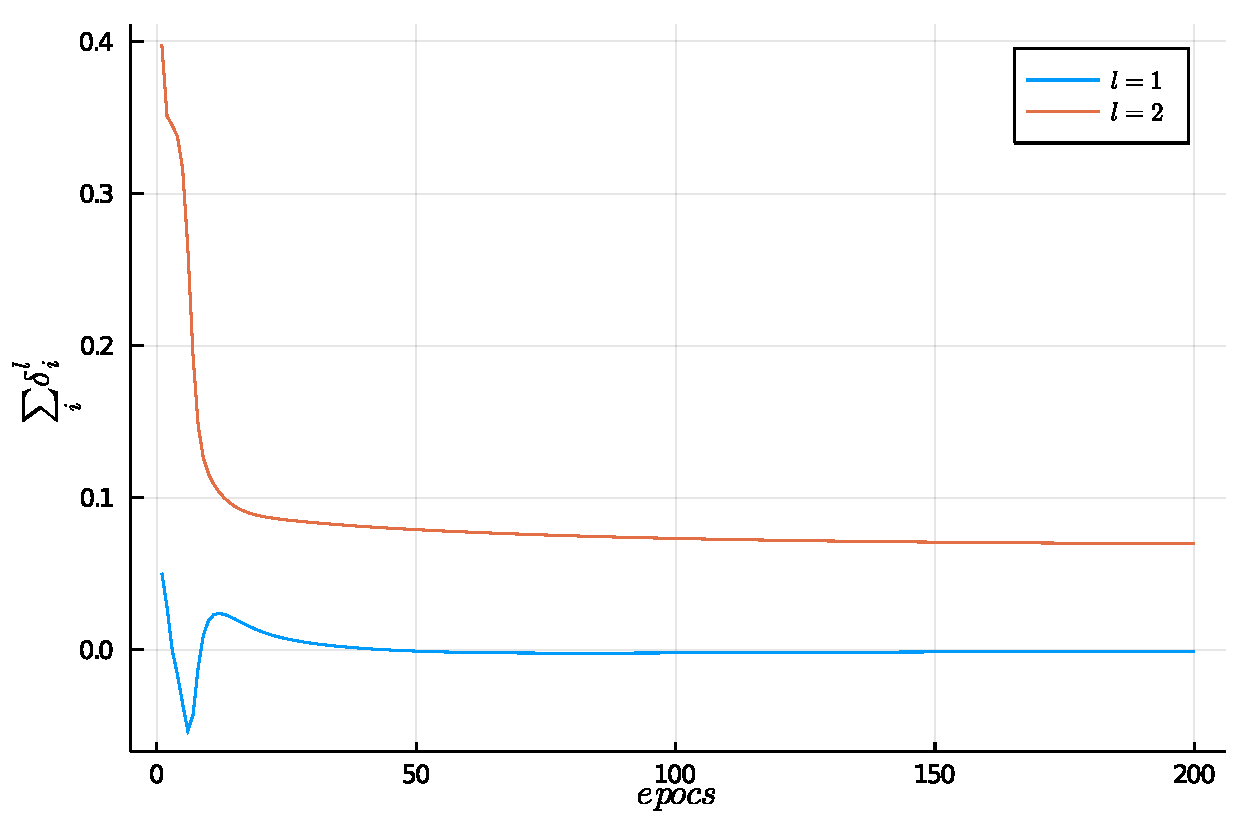
\includegraphics[width=\columnwidth]{figs/gradients-encoder.pdf}
  \caption{Gradients for learning the input data.}
  \label{fig:grad-encoder}
\end{figure}

In spite of this, the data was reduced into the 2-dimensional output of the
hidden layer. This new dataset was then passed into a multilayer perceptron with
1 hidden layer and 3 neurons on this layer (best architecture from past works).
One network was trained using the complete dataset and another using the reduced
one. The results of the classification of the synthesized data are presented in
Fig. \ref{fig:grad-encoder}, where one can observe that some points seem to be
misclassified.

\begin{figure}
  \centering 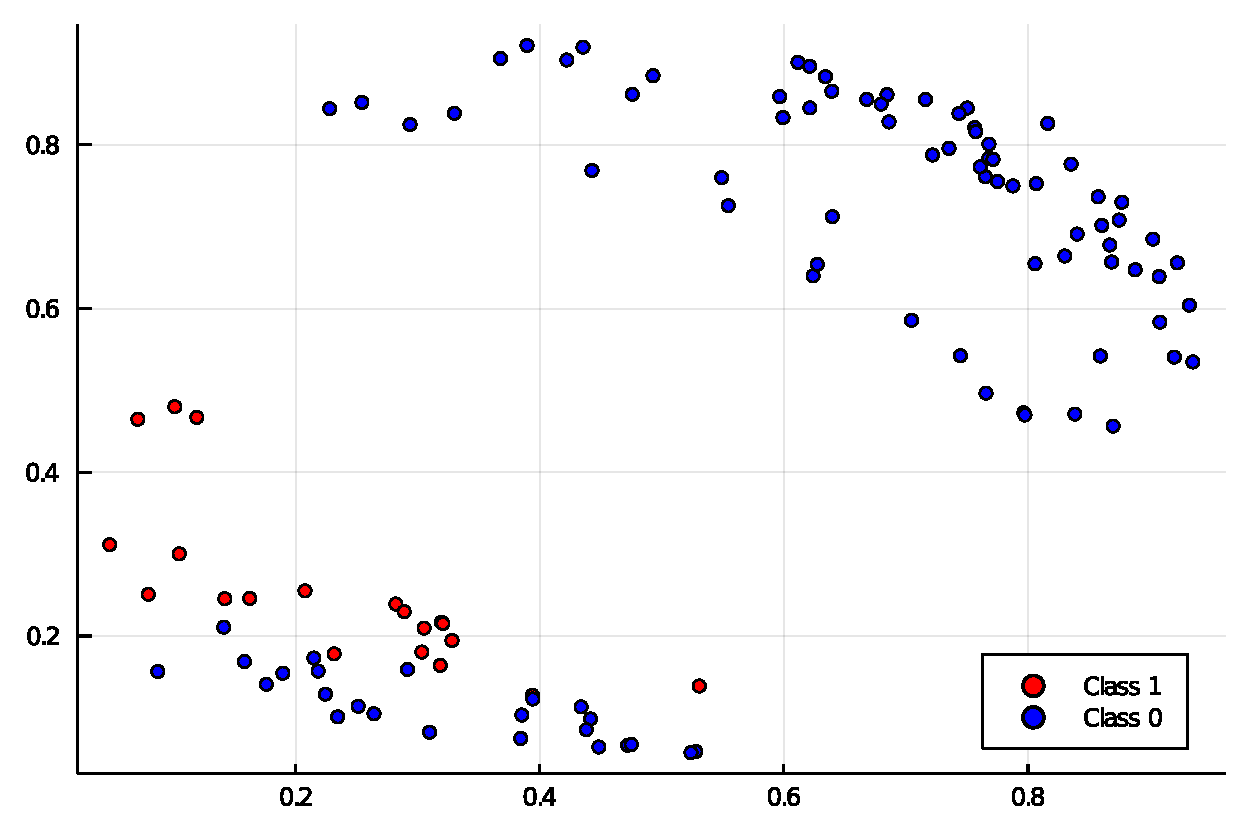
\includegraphics[width=\columnwidth]{figs/reduced-dim-data.pdf}
  \caption{Data projection in 2D using the trained autoencoder.}
  \label{fig:red-data}
\end{figure}

Furthermore, the training curves for the neural network in high dimensions
(original data) are presented in Fig. \ref{fig:high-dims}. Note that the average
error energy is descending fast and the gradients seem to be converging to
zeros. However, Fig. \ref{fig:reduced-dims} shows the learing curves for the
data in reduced by means of the autoencoder and it can be observed that the
gradients are still far from converging to the optimal point and the average
error energy is not decreasing as fast as for the data in high dimensions. This
implies that the classifier works better in high dimensions, at least for 50
epochs.

\begin{figure}
  \centering
  \begin{subfigure}[b]{0.45\textwidth}
    \centering 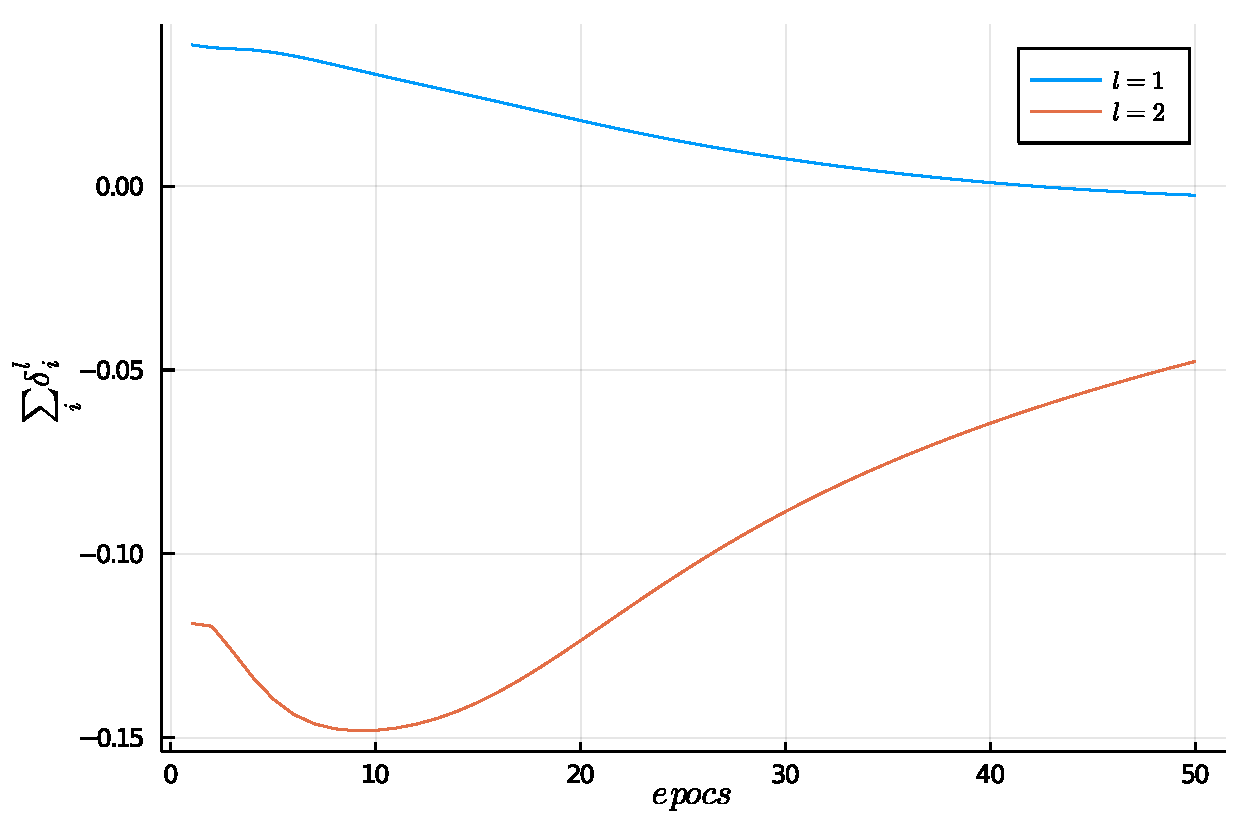
\includegraphics[width=0.9\textwidth]{figs/grads-learn-data.pdf}
    \caption{Training gradients.}
  \end{subfigure}
    %
  \begin{subfigure}[b]{0.45\textwidth}
    \centering
    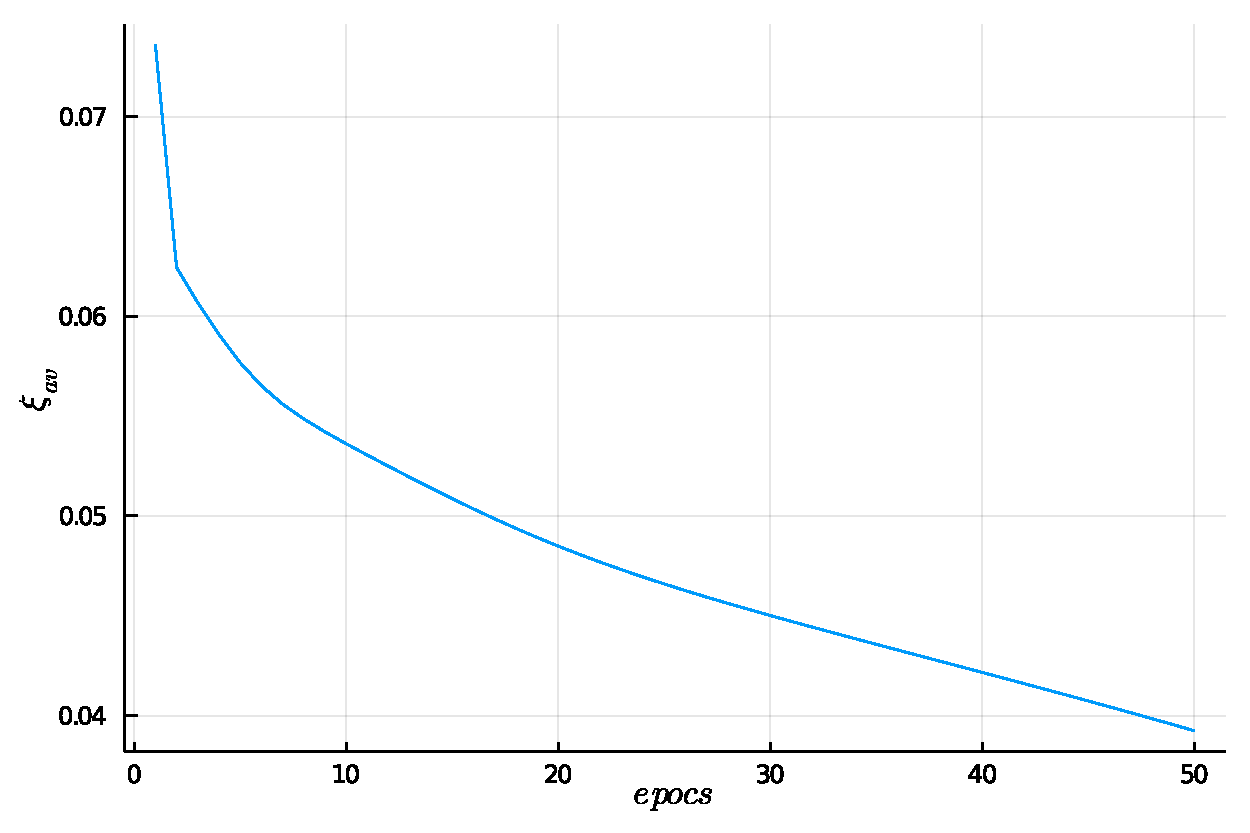
\includegraphics[width=0.9\textwidth]{figs/avg-err-learn-data.pdf}
    \caption{Training average error.}
  \end{subfigure}
  \caption{High dimensional dataset.}
  \label{fig:high-dims}
\end{figure}

\begin{figure}
  \centering
  \begin{subfigure}[b]{0.45\textwidth}
    \centering
    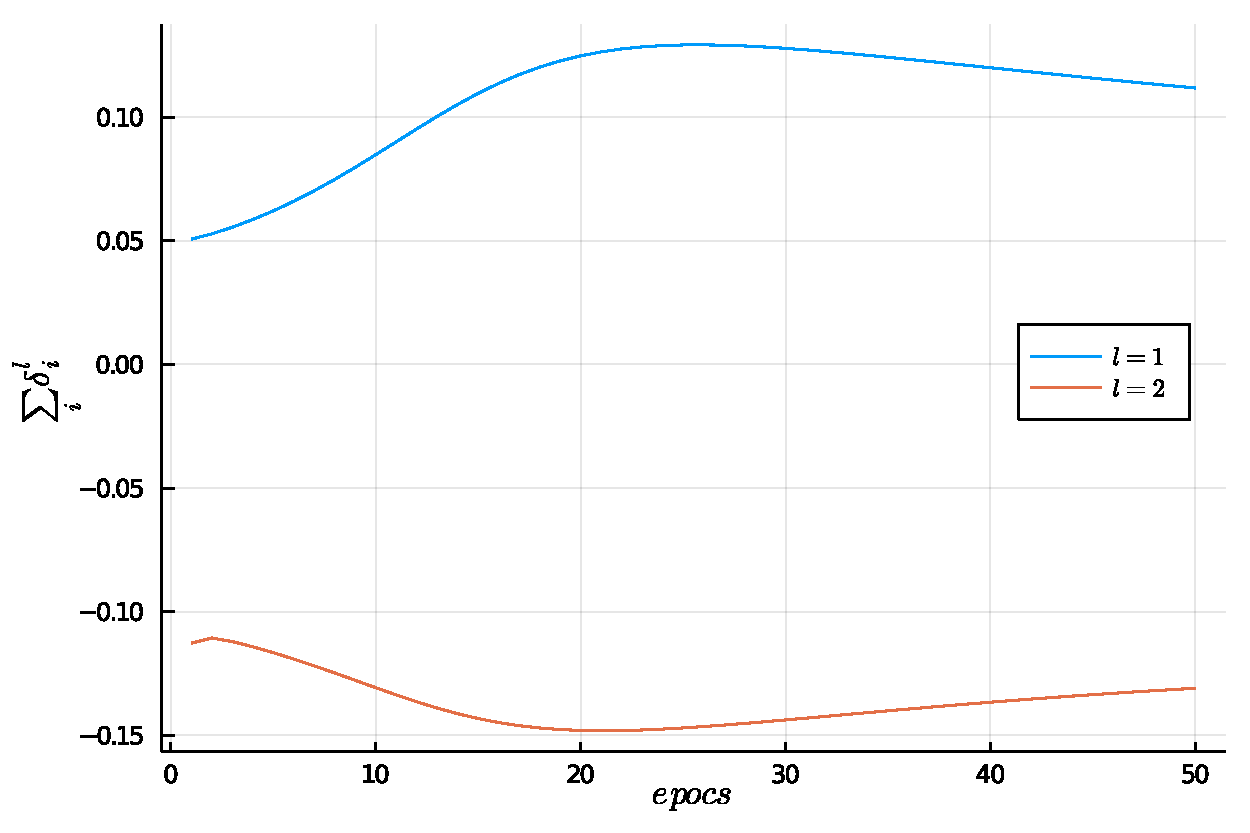
\includegraphics[width=0.9\textwidth]{figs/grads-learn-data-reduced.pdf}
    \caption{Training gradients the reduced dataset.}
  \end{subfigure}
    %
  \begin{subfigure}[b]{0.45\textwidth}
    \centering
    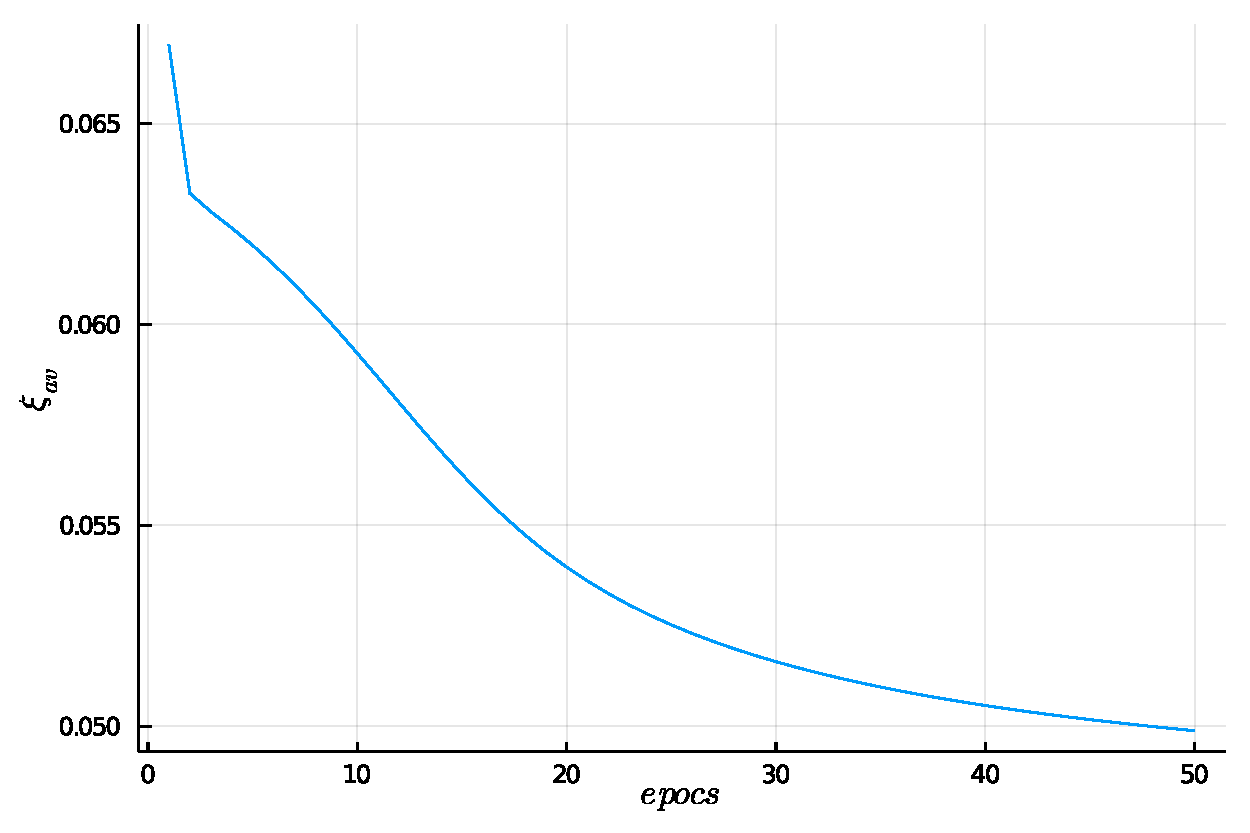
\includegraphics[width=0.9\textwidth]{figs/avg-err-learn-data-reduced.pdf}
    \caption{Training average error the reduced dataset.}
  \end{subfigure}
  \caption{Reduced dataset.}
  \label{fig:reduced-dims}
\end{figure}

\subsection{LeNet5}

As mentioned in the previous section, this architecture was tested using the
LeNet5 architecture. For the training, a pure gradient descent approach was used
with an $\eta = 0.01$ and $200$ epochs. Furthermore, to accelerate training
\texttt{CUDA} was used yielding a 2 second time of execution per epoch. This
allowed to train the network several times and quickly test how to tune the
hyperparameters of the training.

In Table \ref{tab:scores} the scores for the LeNet5 network after training can
be found. This scores were calculated using only the testing dataset in order to
understand if the network could generalize to other points outside the dataset.
It is seen that the architecture was able to successfully generalize most of the
testing dataset; furthermore, this generalization would be improved with a more
detailed revision in the hyperparameters of training without significantly
changing the time of execution.

\begin{table}
  \centering
  \begin{tabular}{cc}
    \hline
    $F_1$ Score & 0.977 \\
    Accuracy    & 0.977 \\ \hline
  \end{tabular}
  \caption{Performance metrics for LeNet5 using testing MNIST dataset.}
  \label{tab:scores}
\end{table}

After understanding that the architecture had successfully generalized over the
testing dataset, it was relevant to understand how the network was able to
classify each of the new data points. In this manner, in Fig.
\ref{fig:lenet5-acts} the activation spaces of the first four layers can be
seen. As each of this activation spaces contained more than 1 feature, the mean
of each of the features per layer was calculated to get a basic idea of how
LeNet5 worked. This activation spaces were extracted using as input the Fig.
\ref{fig:input-act}.

\begin{figure}
  \centering 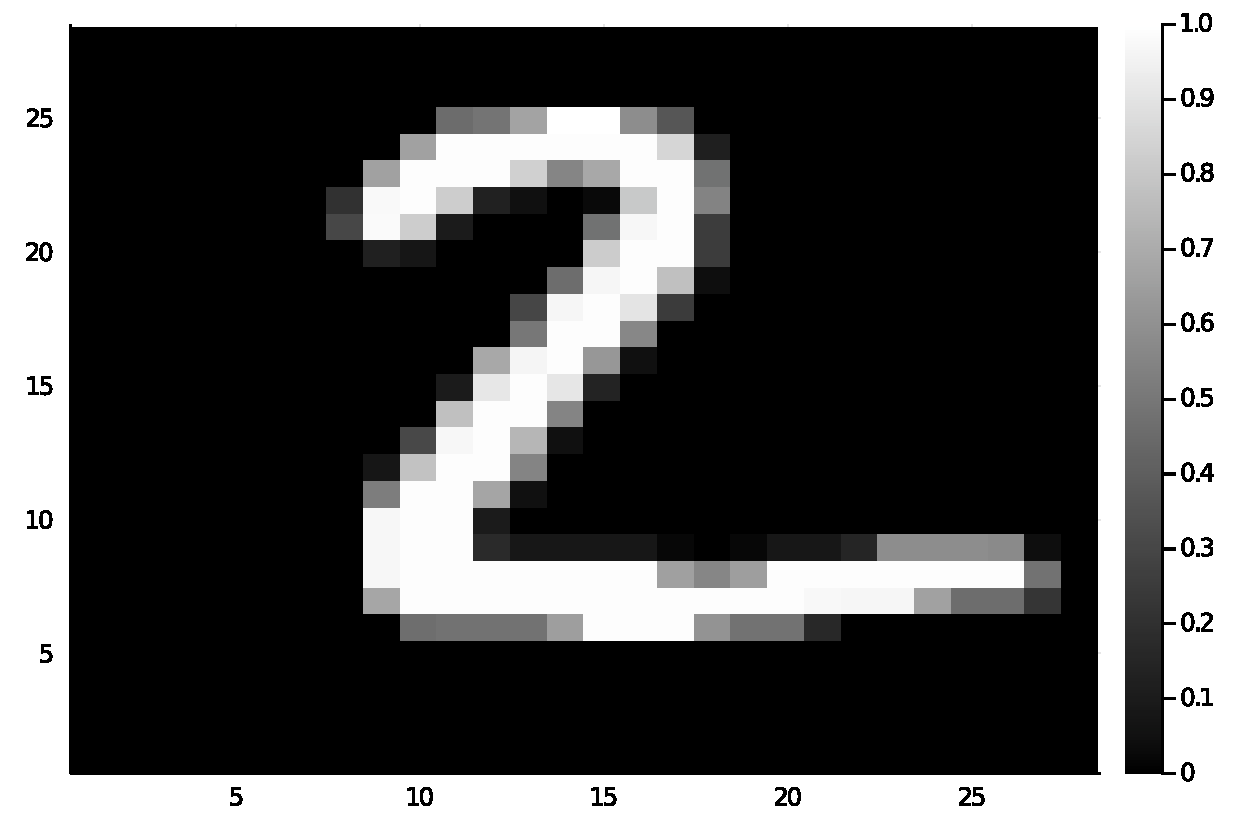
\includegraphics[width=\columnwidth]{figs/input-act-space.pdf}
  \caption{Input for extracting the activation spaces.}
  \label{fig:input-act}
\end{figure}

Some important details arose when analyzing each of the activation spaces. In
the first place, the first layer and second layer were responsible of removing
the basic fodder that the handwritten digit contained. In this manner, after
these two layers a simplified representation of the number was obtained. This is
pretty useful for removing unneeded information such as the caligraphy of the
person who wrote it and so fourth.

In the second place, the other layers zoom in the digit to find any distinctive
curve that could separate the number from the others. This would allow to
recognize small details that human use to recognize handwritten digits and find
out which class does the digit belong to. It is important to remark that this
analysis could be extended using more samples.

\begin{figure*}
  \centering
  \begin{subfigure}[b]{0.45\textwidth}
    \centering 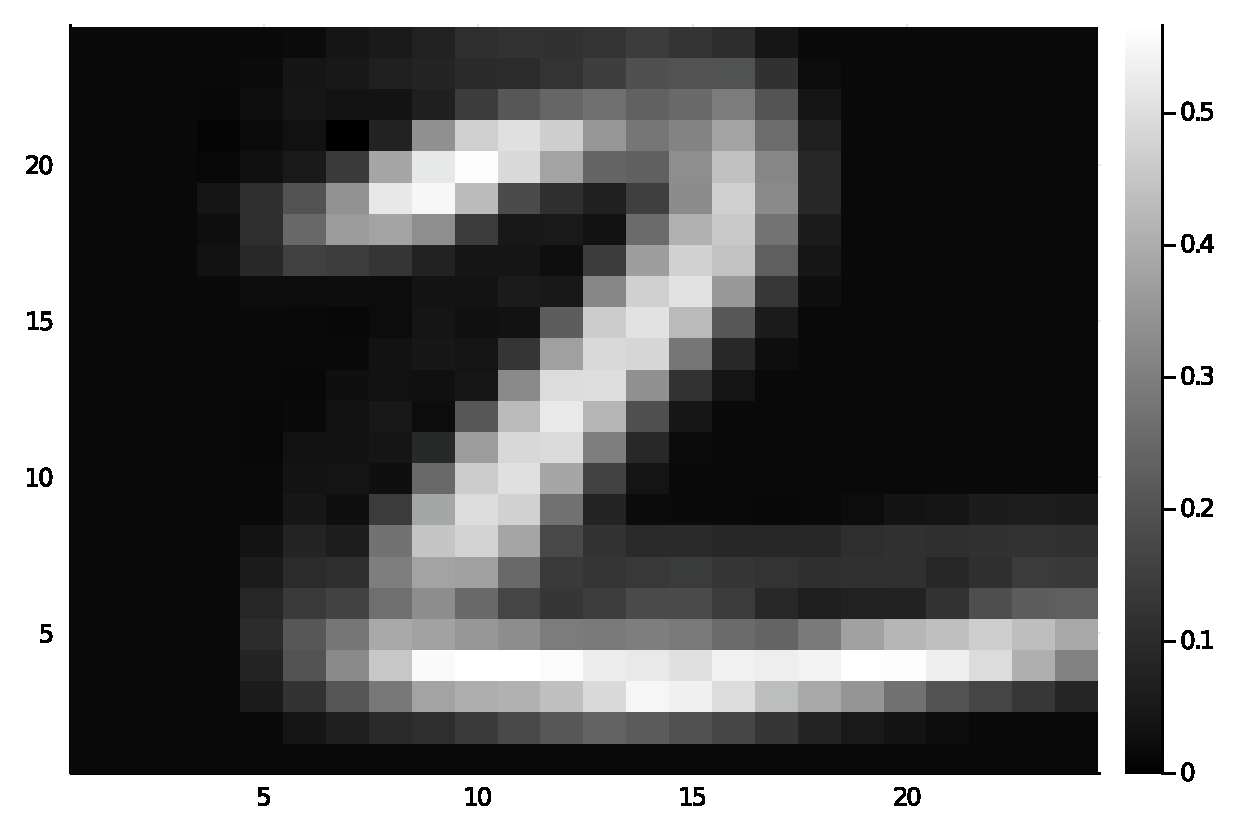
\includegraphics[width=0.9\textwidth]{figs/act-space-1.pdf}
    \caption{Activation space of first layer.}
  \end{subfigure}
    %
  \begin{subfigure}[b]{0.45\textwidth}
    \centering 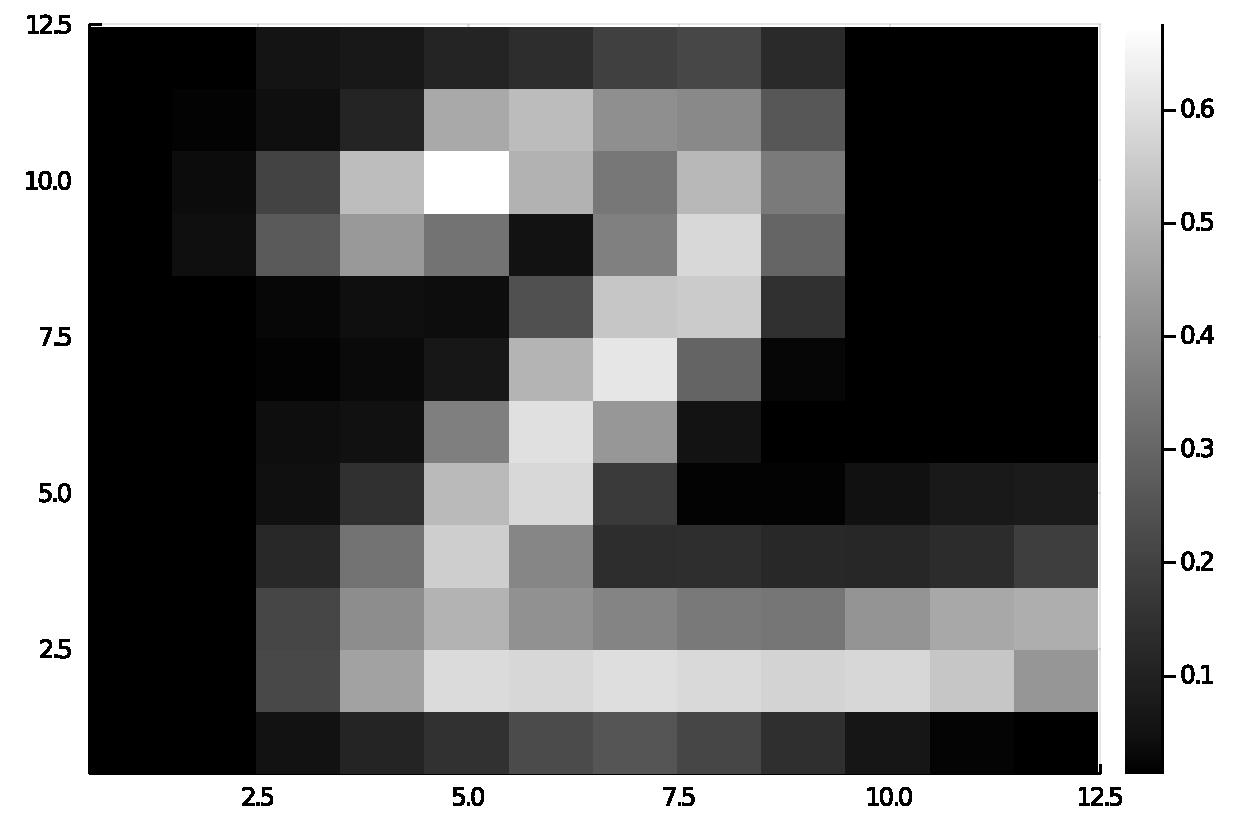
\includegraphics[width=0.9\textwidth]{figs/act-space-2.pdf}
    \caption{Activation space of second layer.}
  \end{subfigure}

  \begin{subfigure}[b]{0.45\textwidth}
    \centering 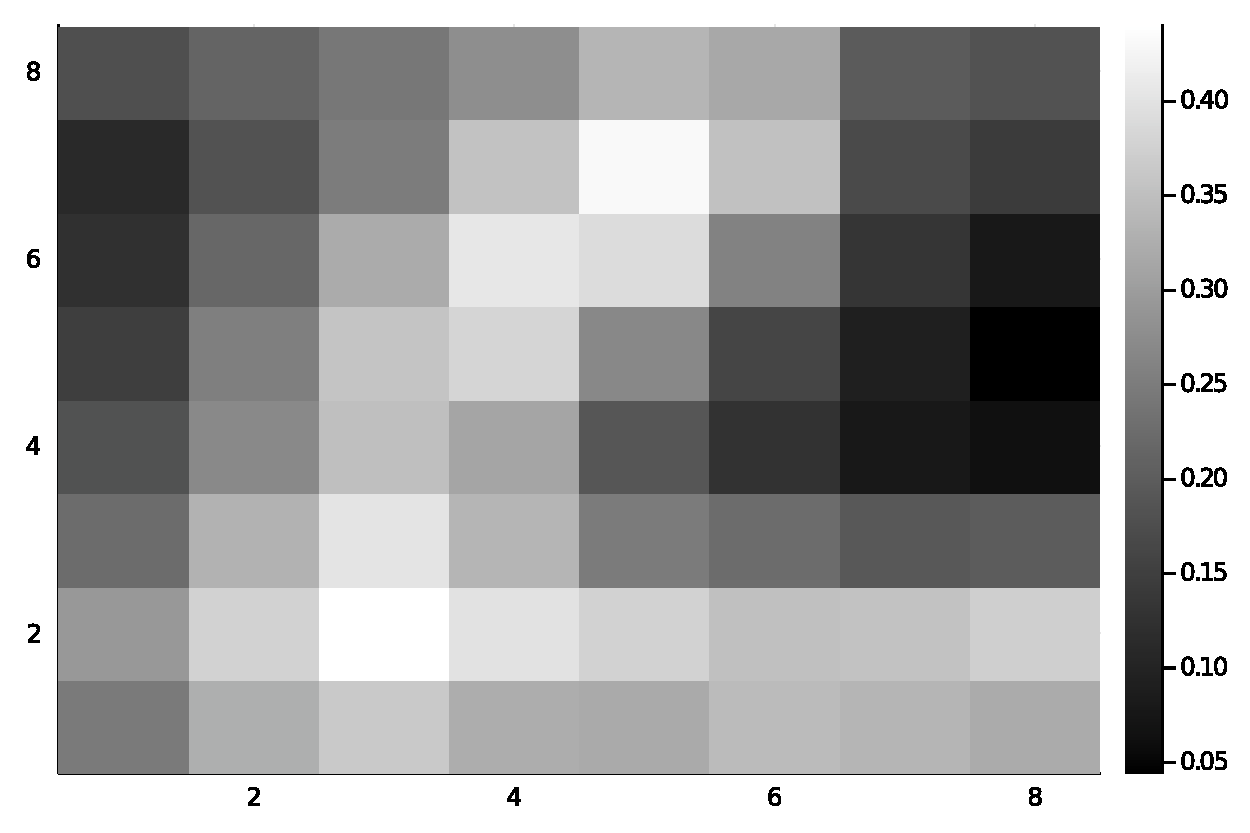
\includegraphics[width=0.9\textwidth]{figs/act-space-3.pdf}
    \caption{Activation space of third layer.}
  \end{subfigure}
    %
  \begin{subfigure}[b]{0.45\textwidth}
    \centering 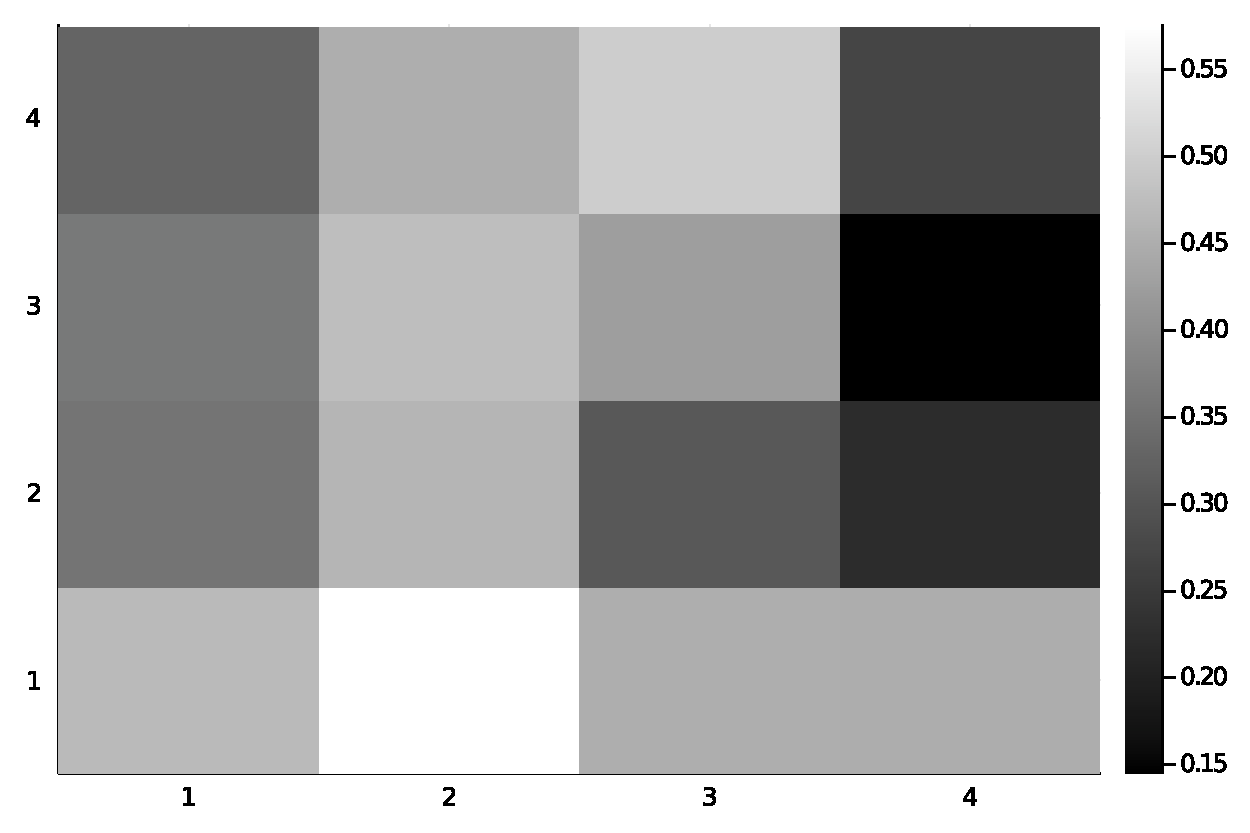
\includegraphics[width=0.9\textwidth]{figs/act-space-4.pdf}
    \caption{Activation space of fourth layer.}
  \end{subfigure}
  \caption{Activation spaces for LeNet5 architecture.}
  \label{fig:lenet5-acts}
\end{figure*}

Lastly, although is useful to see and understand a little bit about this
activation spaces the LeNet5 architecture is still a black box model. In this
manner, it is almost impossible to fully comprehend how the architecture
connects itself and classifies the digits. In this manner, it is still a mystery
to the authors how this works, specially in the last two layers that information
is flattened into fully connected layers.


\subsection{GAN for MNIST}
The code used for this experiments was initially done for the Fashion-MNIST
dataset. The authors extended the implementation specifically for the classic
MNIST dataset and added functions for plotting. The training was done using the
60k training subset, the images have 28$\times$28 pixels and only one color
channel. The training was performed using a batch size of 512 images. The
generator was trained using the \texttt{Adam} optimizer with parameters of 0.001
and \texttt{beta\_1}=0.5. The discriminant was trained using the
\texttt{RMSprop} with parameter of 0.005.

The loss functions for both the discriminant and the generator are presented in
Fig. \ref{fig:loss-gan} and the evolution of the generator of the GAN for 150
epochs can be found in \href{https://bit.ly/39QXrvO}{this link.}

\begin{figure}
  \centering 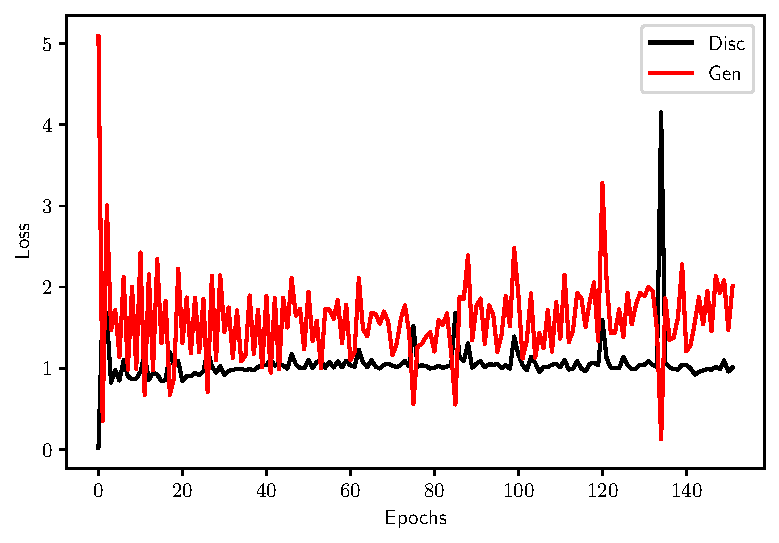
\includegraphics[width=\columnwidth]{figs/loss-GAN.pdf}
  \caption{Loss during training for 150 epochs.}
  \label{fig:loss-gan}
\end{figure}

\subsection{StyleGAN}

For the StyleGAN two different pre-trained networks were used. In first place,
the StyleGAN trained using the classic FFHQ database was used. In Fig.
\ref{fig:grid-ffhq} the style mixing using this StyleGAN network was
constructed. The style mixing is realized by mixing the styles of the images
generated by the StyleGAN of the left column and the upper row. Therefore, it
generates a new set of individuals that have mixed styles.

\begin{figure}
  \centering \includegraphics[width=\columnwidth]{figs/grid-ffhq.png}
  \caption{Style mixing using FFHQ StyleGAN.}
  \label{fig:grid-ffhq}
\end{figure}

It was sup rising to the author's how seamless the mixing of styles was
realized, even taking some aspects from each picture that are not as tangible as
lighting conditions. For example, all the first row of mixed images have that
studio-like lighting; on the other hand, the last row of mixed images preserve
the natural lighting proper of being outside. This features observed by the
StyleGAN are astonishing and highlights the importance of ethics in artificial
intelligence.

In order to test how the FFHQ StyleGAN behaved with other instances of objects
that do not belong originally to the trained data, some other samples were used
to see how the style transfer would do. In this manner, in Fig.
\ref{fig:stylegan-cat} the transfer style for a cat target image can be found.

\begin{figure*}
  \centering
  \begin{subfigure}[b]{0.15\textwidth}
    \centering 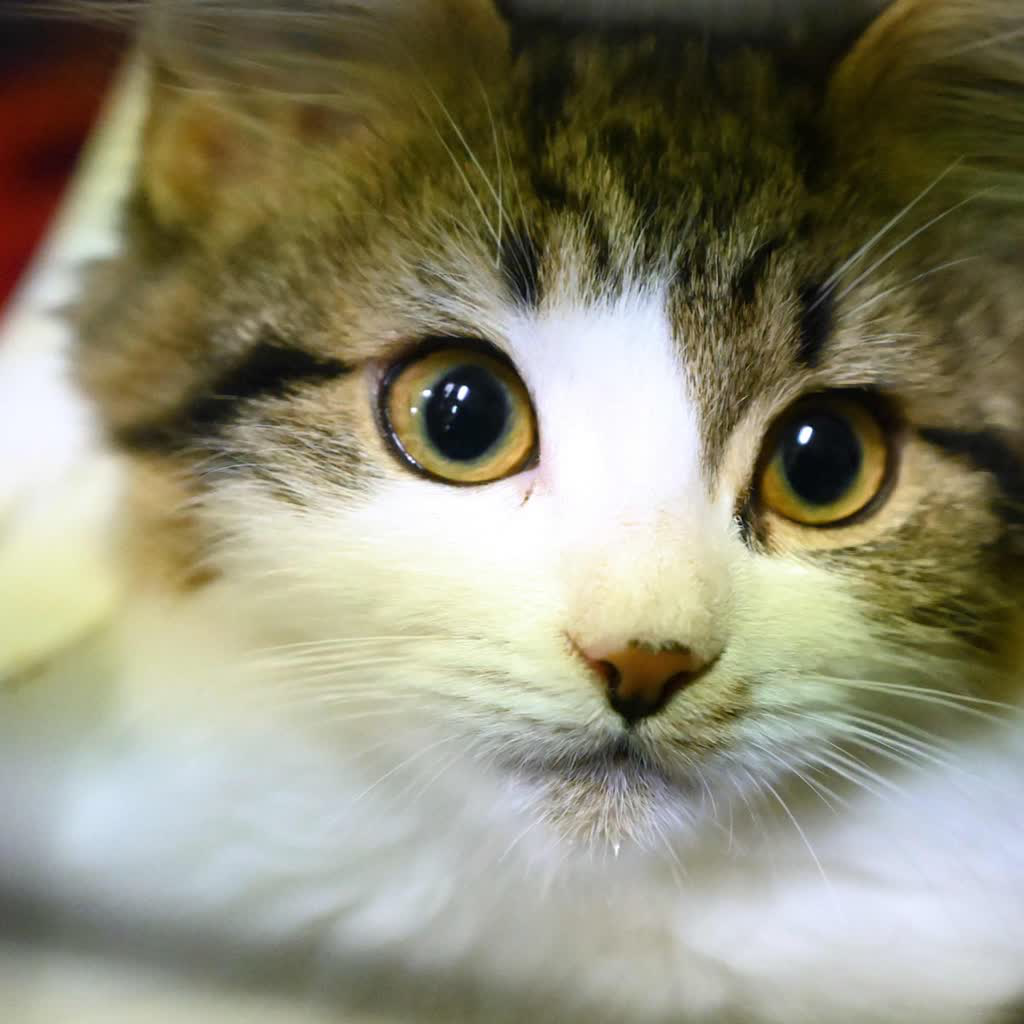
\includegraphics[width=0.9\textwidth]{figs/ffhq-0.png}
    \caption{Target image.}
  \end{subfigure}
  \begin{subfigure}[b]{0.15\textwidth}
    \centering 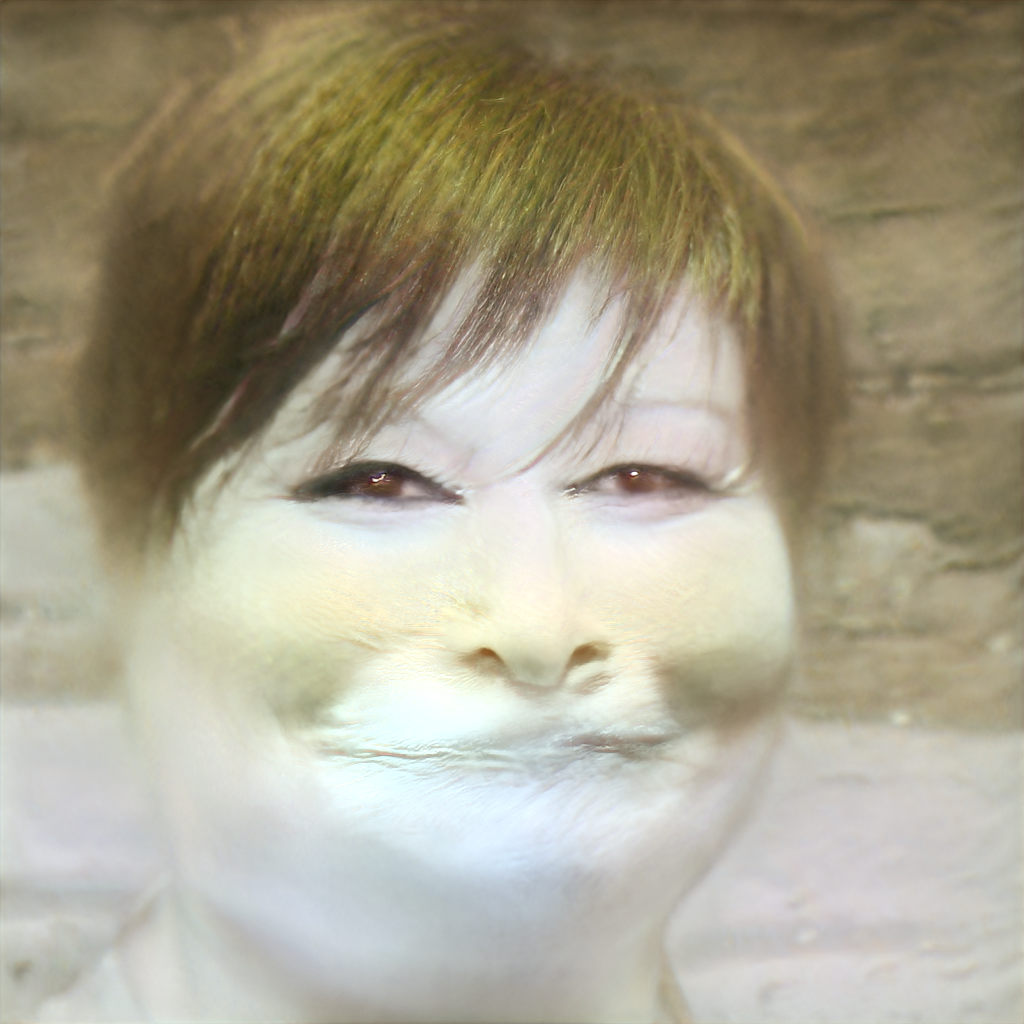
\includegraphics[width=0.9\textwidth]{figs/ffhq-1.png}
    \caption{200 iterations.}
  \end{subfigure}
  \begin{subfigure}[b]{0.15\textwidth}
    \centering 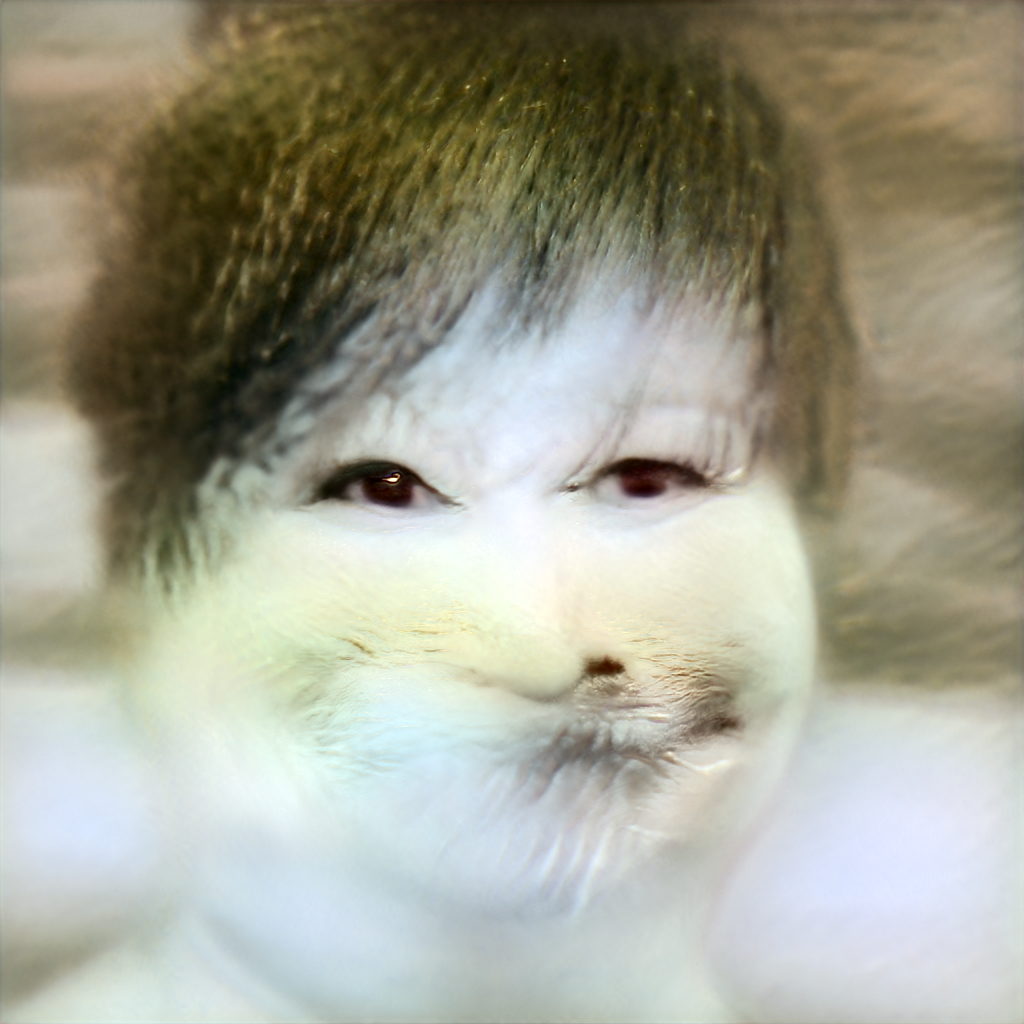
\includegraphics[width=0.9\textwidth]{figs/ffhq-2.png}
    \caption{400 iterations.}
  \end{subfigure}
  \begin{subfigure}[b]{0.15\textwidth}
    \centering 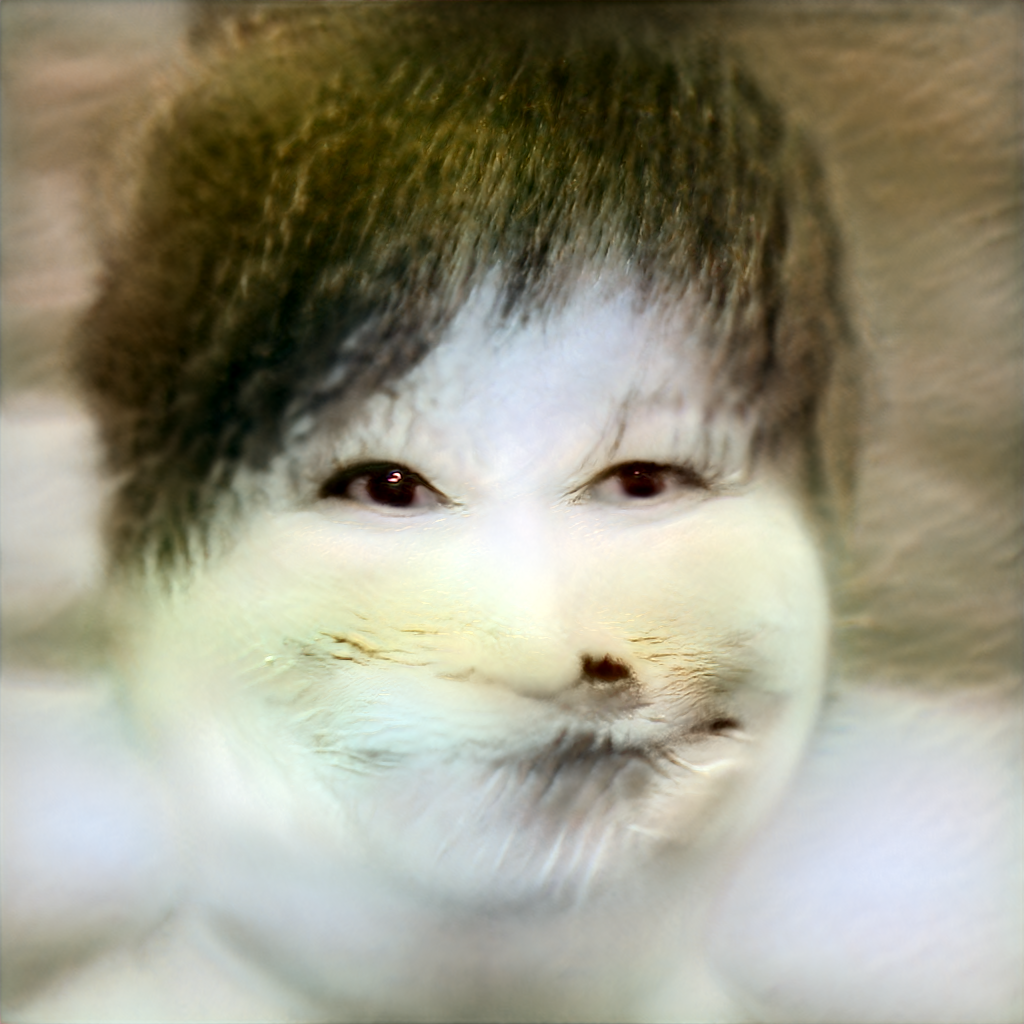
\includegraphics[width=0.9\textwidth]{figs/ffhq-3.png}
    \caption{600 iterations.}
  \end{subfigure}
  \begin{subfigure}[b]{0.15\textwidth}
    \centering 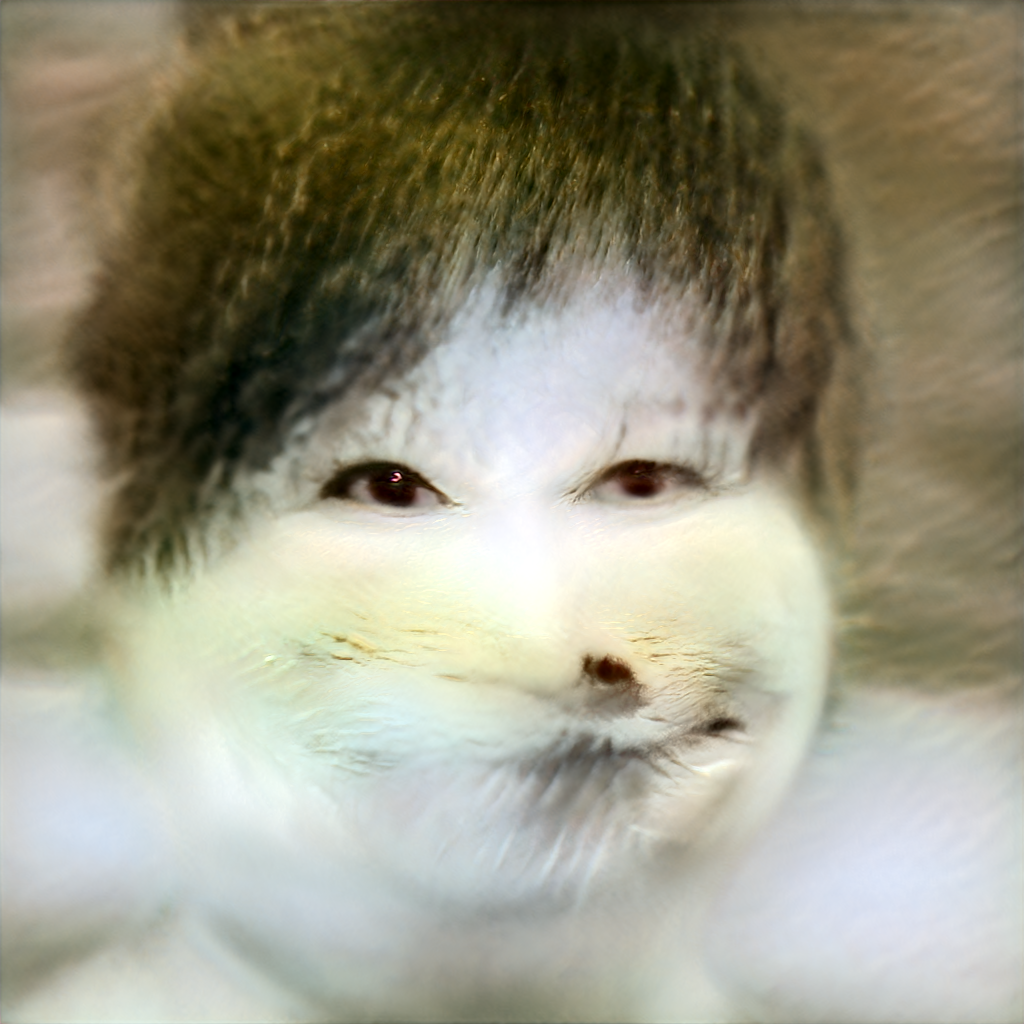
\includegraphics[width=0.9\textwidth]{figs/ffhq-4.png}
    \caption{800 iterations.}
  \end{subfigure}
  \begin{subfigure}[b]{0.15\textwidth}
    \centering 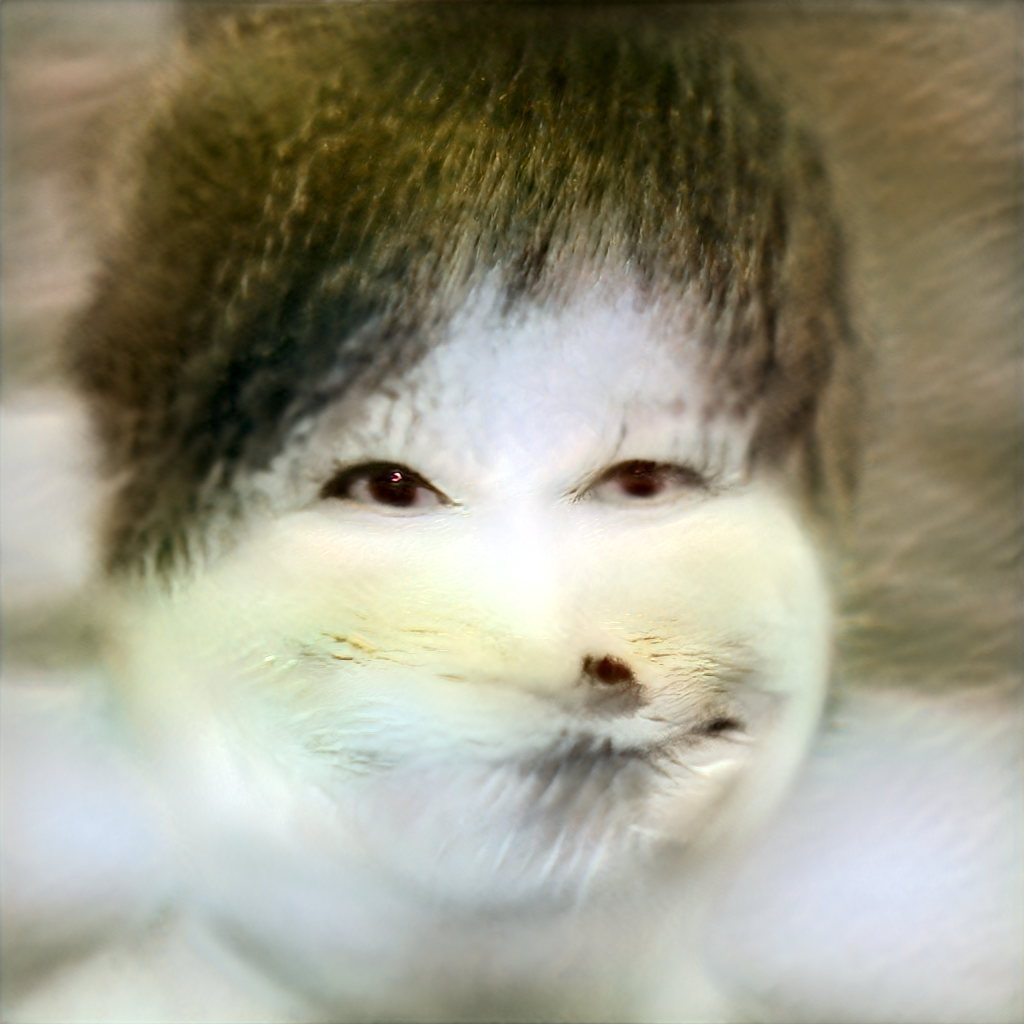
\includegraphics[width=0.9\textwidth]{figs/ffhq-5.png}
    \caption{1000 iterations.}
  \end{subfigure}
  \caption{Transfer style for FFHQ StyleGAN.}
  \label{fig:stylegan-cat}
\end{figure*}

It is seen how, weirdly, attempts to transfer the learn style to a cat that does
not belong to this original style preserving the style of both. In the first
place, it is seen that for more iterations of the network it diverges more from
the original dataset and gets closer to the target image. It is important to
highlight that, at the end, a weird mix is obtained without belonging to any of
the two classes.

To further experiment, the style mixing for an Anime Portrait StyleGAN can be
found in Fig. \label{grid-anime}. This mixing is really interesting as the
StyleGAN has the ability to mix art styles, color schemes and even other
non-tangible characteristics of each of the images.

\begin{figure}
  \centering \includegraphics[width=\columnwidth]{figs/grid-anime.png}
  \caption{Style mixing using Anime Portraits StyleGAN.}
  \label{fig:grid-anime}
\end{figure}

It is really interesting to see the ability of the artificial neural networks to
understand and replicate this kind of art works. Furthermore, this behavior
replicates, similarly, how humans reproduce and create art as many speculate
that human creation comes from a similar process of style mixing. Additionally,
this raises question if human creativity is merely a process of mixing previous
knowledge or comes from true intelligence. In this manner, a kid's drawing is
similar to a not-trained StyleGAN?

This questions will remained unanswered. But the authors think they are of great
importance to fully comprehend human intelligence and it's reach.

In Figs. \ref{fig:ts-anime1}, \ref{fig:ts-anime2} and \ref{fig:ts-anime3} the
transfer styles for the authors and the course teacher can be found
respectively.

\begin{figure*}
  \centering
  \begin{subfigure}[b]{0.15\textwidth}
    \centering 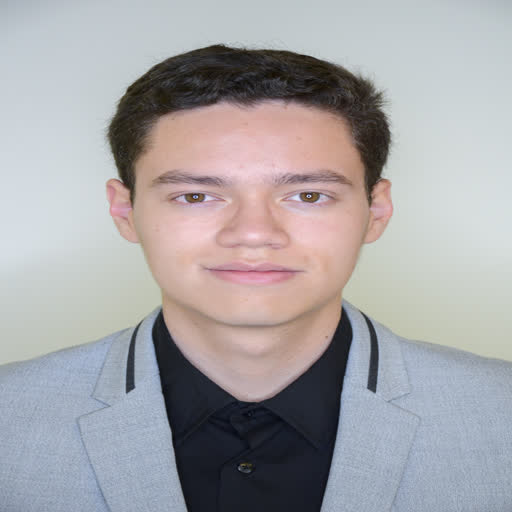
\includegraphics[width=0.9\textwidth]{figs/anime-deipols-0.png}
    \caption{Target image.}
  \end{subfigure}
  \begin{subfigure}[b]{0.15\textwidth}
    \centering 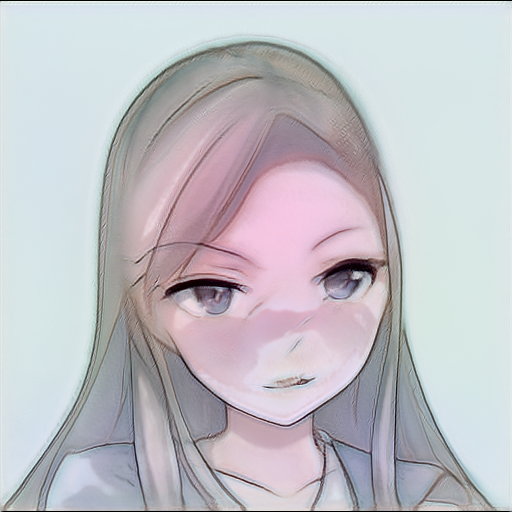
\includegraphics[width=0.9\textwidth]{figs/anime-deipols-1.png}
    \caption{200 iterations.}
  \end{subfigure}
  \begin{subfigure}[b]{0.15\textwidth}
    \centering 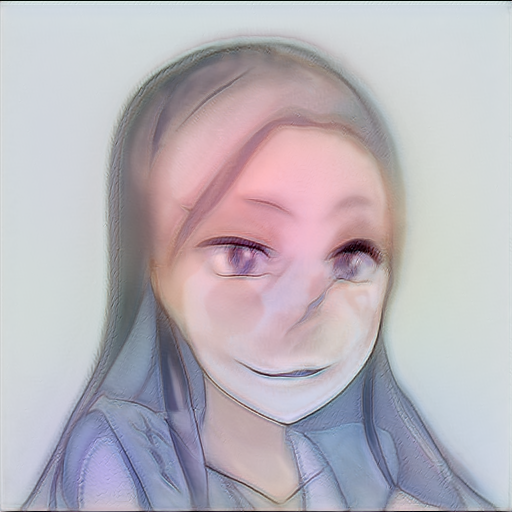
\includegraphics[width=0.9\textwidth]{figs/anime-deipols-2.png}
    \caption{400 iterations.}
  \end{subfigure}
  \begin{subfigure}[b]{0.15\textwidth}
    \centering 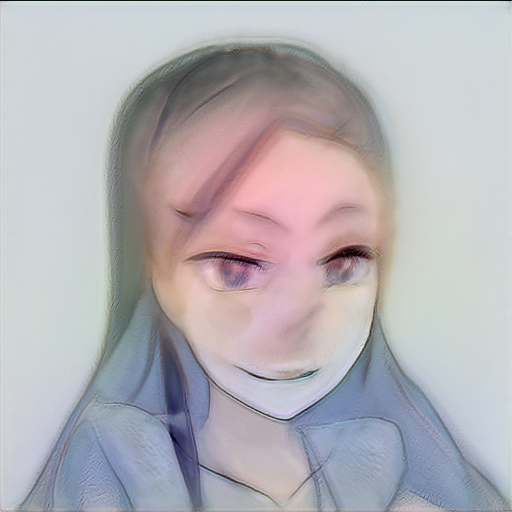
\includegraphics[width=0.9\textwidth]{figs/anime-deipols-3.png}
    \caption{600 iterations.}
  \end{subfigure}
  \begin{subfigure}[b]{0.15\textwidth}
    \centering 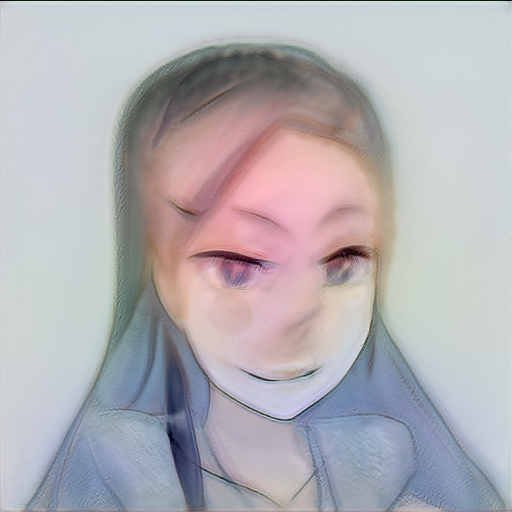
\includegraphics[width=0.9\textwidth]{figs/anime-deipols-4.png}
    \caption{800 iterations.}
  \end{subfigure}
  \begin{subfigure}[b]{0.15\textwidth}
    \centering 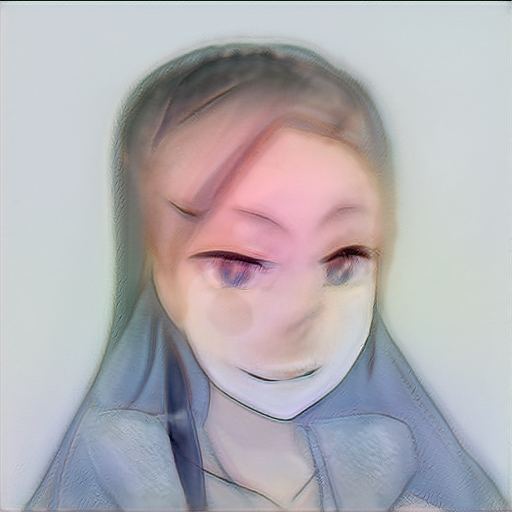
\includegraphics[width=0.9\textwidth]{figs/anime-deipols-5.png}
    \caption{1000 iterations.}
  \end{subfigure}
  \caption{Transfer style for first human test.}
  \label{fig:ts-anime1}
\end{figure*}

\begin{figure*}
  \centering
  \begin{subfigure}[b]{0.15\textwidth}
    \centering 
\includegraphics[width=0.9\textwidth]{figs/anime-js-0.png}
    \caption{Target image.}
  \end{subfigure}
  \begin{subfigure}[b]{0.15\textwidth}
    \centering 
\includegraphics[width=0.9\textwidth]{figs/anime-js-1.png}
    \caption{200 iterations.}
  \end{subfigure}
  \begin{subfigure}[b]{0.15\textwidth}
    \centering 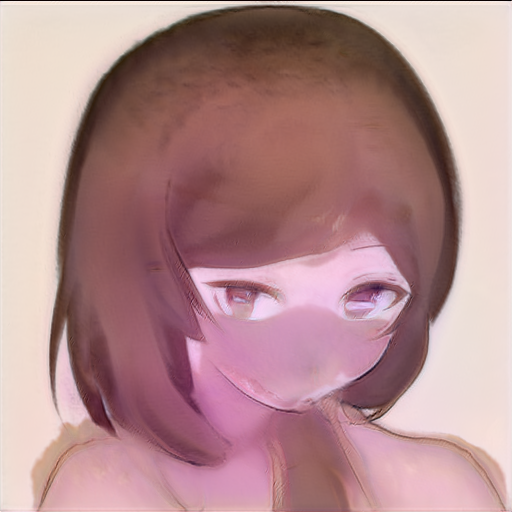
\includegraphics[width=0.9\textwidth]{figs/anime-js-2.png}
    \caption{400 iterations.}
  \end{subfigure}
  \begin{subfigure}[b]{0.15\textwidth}
    \centering 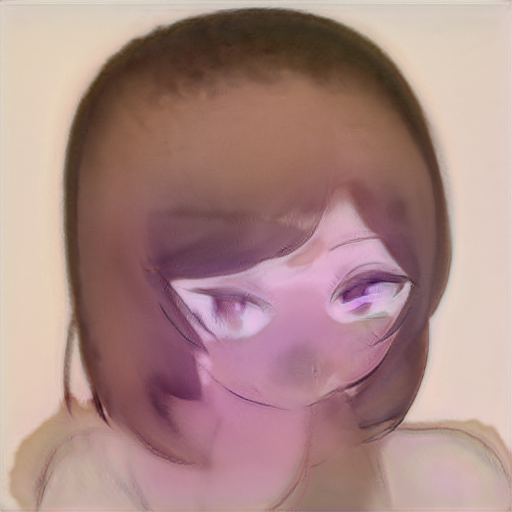
\includegraphics[width=0.9\textwidth]{figs/anime-js-3.png}
    \caption{600 iterations.}
  \end{subfigure}
  \begin{subfigure}[b]{0.15\textwidth}
    \centering 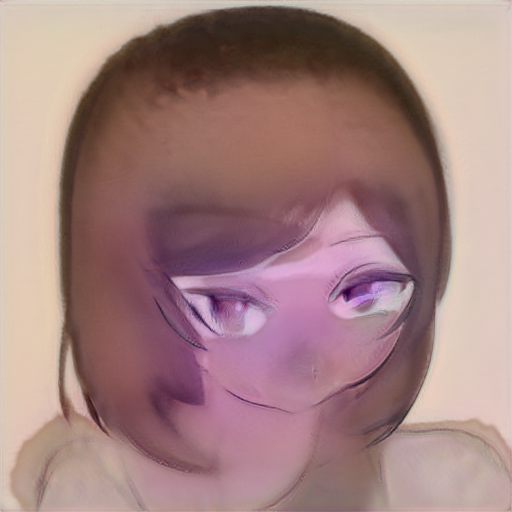
\includegraphics[width=0.9\textwidth]{figs/anime-js-4.png}
    \caption{800 iterations.}
  \end{subfigure}
  \begin{subfigure}[b]{0.15\textwidth}
    \centering 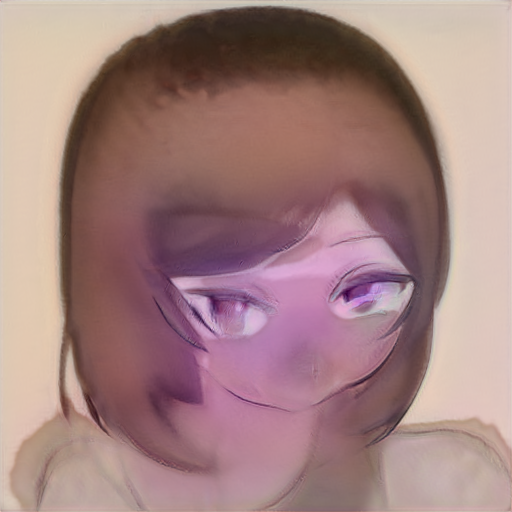
\includegraphics[width=0.9\textwidth]{figs/anime-js-5.png}
    \caption{1000 iterations.}
  \end{subfigure}
  \caption{Transfer style for second human test.}
  \label{fig:ts-anime2}
\end{figure*}

\begin{figure*}
  \centering
  \begin{subfigure}[b]{0.15\textwidth}
    \centering 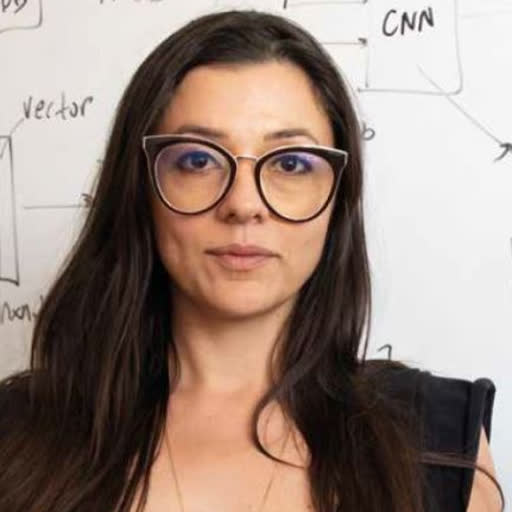
\includegraphics[width=0.9\textwidth]{figs/anime-olga-0.png}
    \caption{Target image.}
  \end{subfigure}
  \begin{subfigure}[b]{0.15\textwidth}
    \centering 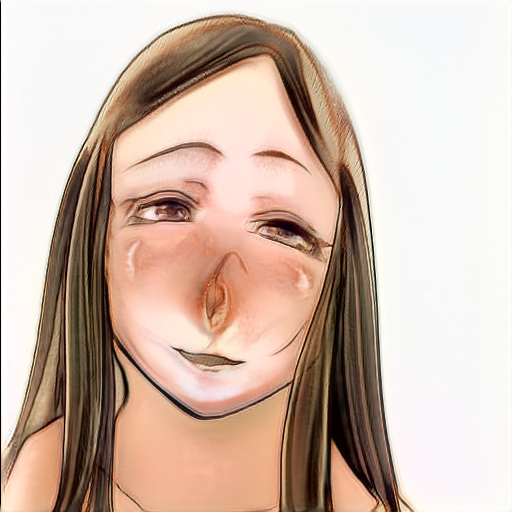
\includegraphics[width=0.9\textwidth]{figs/anime-olga-1.png}
    \caption{200 iterations.}
  \end{subfigure}
  \begin{subfigure}[b]{0.15\textwidth}
    \centering 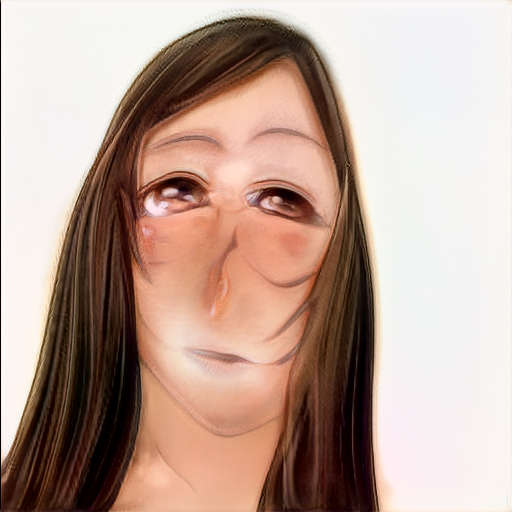
\includegraphics[width=0.9\textwidth]{figs/anime-olga-2.png}
    \caption{400 iterations.}
  \end{subfigure}
  \begin{subfigure}[b]{0.15\textwidth}
    \centering 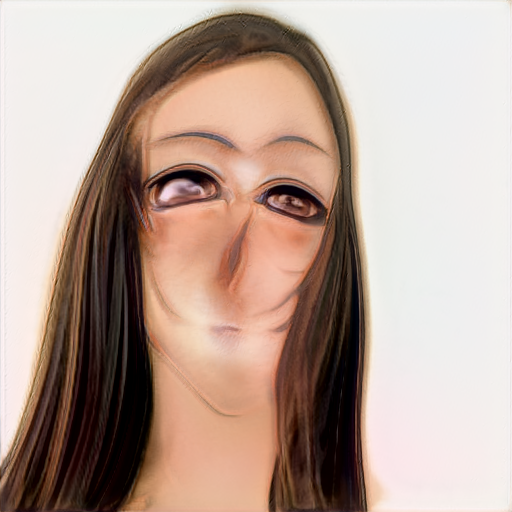
\includegraphics[width=0.9\textwidth]{figs/anime-olga-3.png}
    \caption{600 iterations.}
  \end{subfigure}
  \begin{subfigure}[b]{0.15\textwidth}
    \centering 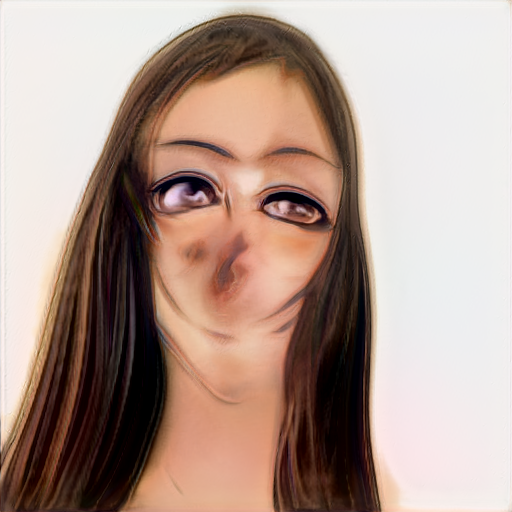
\includegraphics[width=0.9\textwidth]{figs/anime-olga-4.png}
    \caption{800 iterations.}
  \end{subfigure}
  \begin{subfigure}[b]{0.15\textwidth}
    \centering 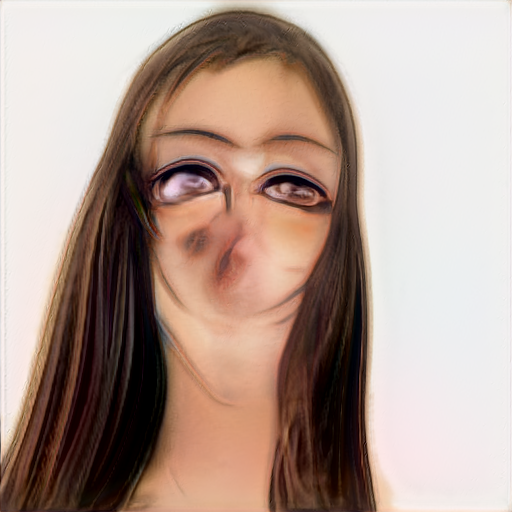
\includegraphics[width=0.9\textwidth]{figs/anime-olga-5.png}
    \caption{1000 iterations.}
  \end{subfigure}
  \caption{Transfer style for third human test.}
  \label{fig:ts-anime3}
\end{figure*}

\section{Conclusions}\label{sec:conc}

This work presented some applications of artificial intelligence techniques in
different contexts. Although all experiments did not give completely successful
results, all of them were implemented and/or used for their specific purpose in
modern environments (\texttt{Python} and \texttt{Julia}) with fairly average
hardware.

First, the autoencoder was successfully implemented and contrasted with the real
high dimensional dataset. Additionally, the LetNet5 architecture was
successfully constructed based on \texttt{Julia}'s libraries and properly
trained for the MNIST dataset in outstanding time (with good performance
measures). Furthermore, the normal GAN architecture was also successfully
trained and evaluated for the MNIST dataset as well. Finally, the StyleGAN was
applied with two different pre-trained networks in both style transfer and style
mixing, with fairly good execution time using personal hardware.

\newpage
\printbibliography

\end{document}
